\documentclass{beamer}
\usepackage{beamerthemesplit}
\usepackage{graphics}
%\usepackage[lined,boxed]{algorithm2e}
\usepackage[lined]{algorithm2e}
\usepackage{amsmath}
\usepackage{amssymb}
\usepackage{listings}
\usepackage{soul}
\usepackage{mathtools}
\newtheorem{thm}{Theorem}
\DeclarePairedDelimiter\ceil{\lceil}{\rceil}
\DeclarePairedDelimiter\floor{\lfloor}{\rfloor}

\lstset{
basicstyle=\small,
keywordstyle=\color{blue}\bfseries,
numbers=left,
numberstyle=\tiny,
numbersep=5pt,
showstringspaces=false,
showspaces=false,
captionpos=b,
frame=tb,
float=tbh,
,escapeinside={*@}{@*}
}
\usetheme{Boadilla}
\title{ Analysis of Algorithms}
\subtitle{Greedy Strategy}
\author{Hikmat Farhat}
%\email{hfarhat@ndu.edu.lb}
%\institution{Notre Dame University}
\newtheorem{mydef}{Definition}
\newtheorem{lem}{Lemma}
%\newcommand{\emphasis}[1]{\textcolor{yellow}{#1}}
%\newcommand{\emphasis}[1]{\hl{#1}}
\newcommand{\emphasis}[1]{\ul{#1}}
%\newcommand{\floor}[1]{\lfloor{#1}\rfloor}
%\newcommand{\bfloor}[1]{\Big\lfloor{#1}\Big\rfloor}

%\newcommand{\gets}[0]{\leftarrow}

%\newcommand{\gets}{\ensuremath{\leftarrow}}
%\DeclareTextFontCommand{\emph}{\emphasis}
\sethlcolor{yellow}

\usepackage{tikz}
\begin{document}

% title page
\frame{\titlepage}



\section{Job scheduling}

\begin{frame}
  \frametitle{Job Scheduling}
  \begin{itemize}
  \item Assume we have $n$ jobs, each with weight $w_i$ and length $l_i$, $1\le i\le n$.
  \item The jobs share some resource (i.e. CPU) so we run them in a consecutive manner.
  \item If we run the jobs in the order $1,2,3,\dots$ then job $i$ has completion time $c_i=\sum_{k=1}^{i}l_k$.
  \item our goal is to minimize the quantity $f=\sum_{k=1}^n w_k\cdot c_k$
  \item In particular, we would like to have a greedy algorithm that minimizes $f$.
  \item To do that we start by looking at special cases
  \end{itemize}
\end{frame}
\begin{frame}
  \frametitle{Special case 1}
  \begin{itemize}
  \item In this special case we assume that all jobs have the same weight then
  \begin{align*}
f&=w(l_1+(l_1+l_2)+(l_1+l_2+l_3)+\ldots +(l_1+\dots+l_n))\\
 &=w(n\cdot l_1+(n-1)\cdot l_2+(n-2)\cdot l_3+\ldots +1\cdot l_n)
\end{align*}
\item Clearly $f$ will be minimized if we choose $l_1\le l_2\le\ldots\le l_n$
  \end{itemize}
\end{frame}
\begin{frame}
  \frametitle{Special case 2}
  \begin{itemize}
  \item The second special case is when all jobs have the same length $l$ then
    \begin{align*}
      f=l(w_1+2\cdot w_2+3\cdot w_3+\ldots n\cdot w_n)
    \end{align*}
\item Clearly, $f$ will be minimized if $w_1\ge w_2\ge w_3\ge\ldots\ge w_n$
  \end{itemize}
\end{frame}
\begin{frame}
  \frametitle{looking for the general case}
  \begin{itemize}
    \item It seems that $f$ increases with $w$ and decreases with $l$.
   \item we need a combination that behaves the same
  \item we can try $w_i-l_i$ and $w_i/l_i$
  \item Which one should be choose?
  \item We try another special case
  \item Suppose we have only two jobs: $w_1=2$, $l_1=1$ and $w_2=6$,$l_2=4$.
  \item if we choose $f=w-l$ then $f_1=1$ and $f_2=2$ this means that job 2 will start first and we get
  \item $6\times 4+2\times 5=34$.
  \item if we choose $f=w/l$ then $f_1=2$ and $f_2=1.5$ this means that job 1 will start first and we get
  \item $2\times 1+6\times 5=32$. Therefore the first method does not lead always to the optimal solution.
  \item Does the second method lead to the optimal solution?
  \end{itemize}
\end{frame}

\begin{frame}
  \frametitle{Proof by exchane argument}
  \begin{itemize}
  \item Let $\sigma$ be an optimal sequence of jobs which is \textbf{ not} greedy.
  \item Since $\sigma$ is not greedy then it contains consecutive jobs $i,k$ such that $w_i/l_i<w_k/l_k$.
   \item we can write 
     \begin{align*}
       X_\sigma=\sum_{j\ne i,k}w_j\cdot c_j+w_i\cdot c_i+w_k\cdot c_k
     \end{align*}
\item Let $\sigma_1$ be the sequence obtained from $\sigma$ by exchanging the order of $i$ and $k$.
\item It is clear that the completion time of all jobs other than $i$ and $k$ remains unchanged. Let $c$ be the sum of completion times of all jobs occurring before $i$ then in the sequence $\sigma$ we have $c_i=c+l_i$ and $c_k=c+l_i+l_k$
  \end{itemize}
\end{frame}
\begin{frame}
  \begin{itemize}
  \item In the sequence $\sigma_1$ we have $c_i=c+l_i+l_k$ and $c_k=c+l_k$.
  \item Then
  \end{itemize}
  \begin{align*}
    X_\sigma-X_{\sigma_1}&=(w_i\cdot c+w_i\cdot l_i+w_k\cdot c+w_k\cdot l_i+w_k\cdot l_k)\\
                      &-(w_i\cdot c+w_i\cdot l_i+w_i\cdot l_k+w_k\cdot c+w_k\cdot l_k)\\
                      &=w_k\cdot l_i-w_i\cdot l_k>0\\
                      &\Rightarrow X_\sigma>X_{\sigma_1}
  \end{align*}
  \begin{itemize}
  \item The last two lines follow from  $w_i/l_i<w_k/l_k\Rightarrow w_i\cdot l_k <w_k\cdot l_i$.
  \item This is a contradiction because $\sigma$ was assumed to be optimal.
  \end{itemize}
\end{frame}
\section{Scheduling}
\begin{frame}
  \frametitle{Interval Scheduling}
  \begin{itemize}
    \item Consider a set of $n$ intervals $(s,e)$ where $s$ and $e$ are the starting and ending time respectively.
    \item We would like to choose a non-overlapping subset of those intervals such that the total number of selected intervals is maximum.
    \item For example, consider the intervals $\{(1,5),(2,7),(5,8)\}$. The largest subset of non-overlapping intervals is $\{(1,5),(5,8)\}$. 

  \end{itemize}
    
We are looking for a greedy solution to this optimization problem. What property of the intervals should the greedy method select? There are many options:
\begin{enumerate}
  \item shortest interval first
  \item The interval with the smallest starting time
  \item The interval with the smalles number of overlaps 
  \item etc...
\end{enumerate}
\end{frame}
\begin{frame}
  \frametitle{Shortest iterval first}
\ifx\du\undefined
  \newlength{\du}
\fi
\setlength{\du}{15\unitlength}

\begin{figure}[h]
  \centering

\begin{tikzpicture}
\pgftransformxscale{1.000000}
\pgftransformyscale{-1.000000}
\definecolor{dialinecolor}{rgb}{0.000000, 0.000000, 0.000000}
\pgfsetstrokecolor{dialinecolor}
\definecolor{dialinecolor}{rgb}{1.000000, 1.000000, 1.000000}
\pgfsetfillcolor{dialinecolor}
\pgfsetlinewidth{1.000000\du}
\pgfsetdash{}{0pt}
\pgfsetdash{}{0pt}
\pgfsetbuttcap
{
\definecolor{dialinecolor}{rgb}{0.498039, 0.498039, 0.498039}
\pgfsetfillcolor{dialinecolor}
% was here!!!
\definecolor{dialinecolor}{rgb}{0.498039, 0.498039, 0.498039}
\pgfsetstrokecolor{dialinecolor}
\draw (8.100000\du,-6.300000\du)--(12.300000\du,-6.30000\du);
}
\pgfsetlinewidth{1.000000\du}
\pgfsetdash{}{0pt}
\pgfsetdash{}{0pt}
\pgfsetbuttcap
{
\definecolor{dialinecolor}{rgb}{0.498039, 0.498039, 0.498039}
\pgfsetfillcolor{dialinecolor}
% was here!!!
\definecolor{dialinecolor}{rgb}{0.498039, 0.498039, 0.498039}
\pgfsetstrokecolor{dialinecolor}
\draw (1.650000\du,-4.65000\du)--(9.600000\du,-4.650000\du);
}
\pgfsetlinewidth{1.000000\du}
\pgfsetdash{}{0pt}
\pgfsetdash{}{0pt}
\pgfsetbuttcap
{
\definecolor{dialinecolor}{rgb}{0.498039, 0.498039, 0.498039}
\pgfsetfillcolor{dialinecolor}
% was here!!!
\definecolor{dialinecolor}{rgb}{0.498039, 0.498039, 0.498039}
\pgfsetstrokecolor{dialinecolor}
\draw (11.400000\du,-4.650000\du)--(18.904801\du,-4.65\du);
}
\end{tikzpicture}
  
  \caption{Shortest interval counterexample}
\end{figure}

\end{frame}

\begin{frame}
  \frametitle{Earliest starting time first}
  \ifx\du\undefined
  \newlength{\du}
\fi
\setlength{\du}{15\unitlength}

\begin{figure}[h]
  \centering
  
  
\begin{tikzpicture}
\pgftransformxscale{1.000000}
\pgftransformyscale{-1.000000}
\definecolor{dialinecolor}{rgb}{0.000000, 0.000000, 0.000000}
\pgfsetstrokecolor{dialinecolor}
\definecolor{dialinecolor}{rgb}{1.000000, 1.000000, 1.000000}
\pgfsetfillcolor{dialinecolor}
\pgfsetlinewidth{1.000000\du}
\pgfsetdash{}{0pt}
\pgfsetdash{}{0pt}
\pgfsetbuttcap
{
\definecolor{dialinecolor}{rgb}{0.498039, 0.498039, 0.498039}
\pgfsetfillcolor{dialinecolor}
% was here!!!
\definecolor{dialinecolor}{rgb}{0.498039, 0.498039, 0.498039}
\pgfsetstrokecolor{dialinecolor}
\draw (4.550000\du,-1.90000\du)--(9.350000\du,-1.900000\du);
}
\pgfsetlinewidth{1.000000\du}
\pgfsetdash{}{0pt}
\pgfsetdash{}{0pt}
\pgfsetbuttcap
{
\definecolor{dialinecolor}{rgb}{0.498039, 0.498039, 0.498039}
\pgfsetfillcolor{dialinecolor}
% was here!!!
\definecolor{dialinecolor}{rgb}{0.498039, 0.498039, 0.498039}
\pgfsetstrokecolor{dialinecolor}
\draw (1.650000\du,-4.65000\du)--(14.950000\du,-4.650000\du);
}
\pgfsetlinewidth{1.000000\du}
\pgfsetdash{}{0pt}
\pgfsetdash{}{0pt}
\pgfsetbuttcap
{
\definecolor{dialinecolor}{rgb}{0.498039, 0.498039, 0.498039}
\pgfsetfillcolor{dialinecolor}
% was here!!!
\definecolor{dialinecolor}{rgb}{0.498039, 0.498039, 0.498039}
\pgfsetstrokecolor{dialinecolor}
\draw (10.150000\du,-1.90000\du)--(17.750000\du,-1.900000\du);
}
\end{tikzpicture}
\caption{counterexample for earliest starting time first}
\end{figure}

\end{frame}
\begin{frame}
  \frametitle{Smallest overlap first}
  \ifx\du\undefined
  \newlength{\du}
\fi
\setlength{\du}{15\unitlength}
\begin{figure}
\begin{tikzpicture}
\pgftransformxscale{0.8500000}
\pgftransformyscale{-1.000000}
\definecolor{dialinecolor}{rgb}{0.000000, 0.000000, 0.000000}
\pgfsetstrokecolor{dialinecolor}
\definecolor{dialinecolor}{rgb}{1.000000, 1.000000, 1.000000}
\pgfsetfillcolor{dialinecolor}
\pgfsetlinewidth{1.000000\du}
\pgfsetdash{}{0pt}
\pgfsetdash{}{0pt}
\pgfsetbuttcap
{
\definecolor{dialinecolor}{rgb}{0.000000, 0.000000, 0.000000}
\pgfsetfillcolor{dialinecolor}
% was here!!!
\definecolor{dialinecolor}{rgb}{0.000000, 0.000000, 0.000000}
\pgfsetstrokecolor{dialinecolor}
\draw (3.550000\du,-1.900000\du)--(9.350000\du,-1.900000\du);
}
\pgfsetlinewidth{1.000000\du}
\pgfsetdash{}{0pt}
\pgfsetdash{}{0pt}
\pgfsetbuttcap
{
\definecolor{dialinecolor}{rgb}{0.000000, 0.000000, 0.000000}
\pgfsetfillcolor{dialinecolor}
% was here!!!
\definecolor{dialinecolor}{rgb}{0.000000, 0.000000, 0.000000}
\pgfsetstrokecolor{dialinecolor}
\draw (23.850000\du,-1.955000\du)--(29.650000\du,-1.955000\du);
}
\pgfsetlinewidth{1.000000\du}
\pgfsetdash{}{0pt}
\pgfsetdash{}{0pt}
\pgfsetbuttcap
{
\definecolor{dialinecolor}{rgb}{0.498039, 0.498039, 0.498039}
\pgfsetfillcolor{dialinecolor}
% was here!!!
\definecolor{dialinecolor}{rgb}{0.498039, 0.498039, 0.498039}
\pgfsetstrokecolor{dialinecolor}
\draw (17.050000\du,-1.910000\du)--(22.850000\du,-1.910000\du);
}
\pgfsetlinewidth{1.000000\du}
\pgfsetdash{}{0pt}
\pgfsetdash{}{0pt}
\pgfsetbuttcap
{
\definecolor{dialinecolor}{rgb}{0.498039, 0.498039, 0.498039}
\pgfsetfillcolor{dialinecolor}
% was here!!!
\definecolor{dialinecolor}{rgb}{0.498039, 0.498039, 0.498039}
\pgfsetstrokecolor{dialinecolor}
\draw (10.350000\du,-1.915000\du)--(16.150000\du,-1.915000\du);
}
\pgfsetlinewidth{1.000000\du}
\pgfsetdash{}{0pt}
\pgfsetdash{}{0pt}
\pgfsetbuttcap
{
\definecolor{dialinecolor}{rgb}{0.000000, 0.000000, 0.000000}
\pgfsetfillcolor{dialinecolor}
% was here!!!
\definecolor{dialinecolor}{rgb}{0.000000, 0.000000, 0.000000}
\pgfsetstrokecolor{dialinecolor}
\draw (13.900000\du,-0.070000\du)--(19.700000\du,-0.070000\du);
}
\pgfsetlinewidth{1.000000\du}
\pgfsetdash{}{0pt}
\pgfsetdash{}{0pt}
\pgfsetbuttcap
{
\definecolor{dialinecolor}{rgb}{0.498039, 0.498039, 0.498039}
\pgfsetfillcolor{dialinecolor}
% was here!!!
\definecolor{dialinecolor}{rgb}{0.498039, 0.498039, 0.498039}
\pgfsetstrokecolor{dialinecolor}
\draw (6.800000\du,1.075000\du)--(12.600000\du,1.075000\du);
}
\pgfsetlinewidth{1.000000\du}
\pgfsetdash{}{0pt}
\pgfsetdash{}{0pt}
\pgfsetbuttcap
{
\definecolor{dialinecolor}{rgb}{0.498039, 0.498039, 0.498039}
\pgfsetfillcolor{dialinecolor}
% was here!!!
\definecolor{dialinecolor}{rgb}{0.498039, 0.498039, 0.498039}
\pgfsetstrokecolor{dialinecolor}
\draw (6.800000\du,3.020000\du)--(12.600000\du,3.020000\du);
}
\pgfsetlinewidth{1.000000\du}
\pgfsetdash{}{0pt}
\pgfsetdash{}{0pt}
\pgfsetbuttcap
{
\definecolor{dialinecolor}{rgb}{0.498039, 0.498039, 0.498039}
\pgfsetfillcolor{dialinecolor}
% was here!!!
\definecolor{dialinecolor}{rgb}{0.498039, 0.498039, 0.498039}
\pgfsetstrokecolor{dialinecolor}
\draw (21.250000\du,1.065000\du)--(27.050000\du,1.065000\du);
}
\pgfsetlinewidth{1.000000\du}
\pgfsetdash{}{0pt}
\pgfsetdash{}{0pt}
\pgfsetbuttcap
{
\definecolor{dialinecolor}{rgb}{0.498039, 0.498039, 0.498039}
\pgfsetfillcolor{dialinecolor}
% was here!!!
\definecolor{dialinecolor}{rgb}{0.498039, 0.498039, 0.498039}
\pgfsetstrokecolor{dialinecolor}
\draw (21.250000\du,3.160000\du)--(27.050000\du,3.160000\du);
}
\end{tikzpicture}
\caption{Smallest overlap first}
\end{figure}
\end{frame}

\begin{frame}
  \frametitle{Greedy Solution}
  The greedy solution consists of choose the next compatible interval with the smallest finishing time. We build a min-heap based on finishing times. Let $I$ be the set of intervals and $T$ the desired solution
  \begin{algorithm}[H]
\SetKwFunction{dm}{Delete-Min(Q)}
%\dontprintsemicolon
\DontPrintSemicolon
$Q\gets I$\;
$T\gets\emptyset$\;
$last\gets -1$\;
\While{$Q\ne\emptyset$ }{
$(s,f)\gets \dm$\;

\If{$s\ge last$}{
  $T\gets T\cup\{(s,f)\}$\;
  $last\gets f$\;
}
}

\end{algorithm}
\end{frame}

\begin{frame}
  \begin{itemize}
  \item Let $I$ be the set of intervals. A solution to the interval scheduling is a subset $S=\{s_1,f_1),\ldots,(s_k,f_k)\}\subseteq I$ such that
for all $i<j$ we have $f_i\le s_j$.
\item  Our goal is to find the optimal solution, i.e. the solution with the largest number of intervals.
\item We will show that the greedy solution is optimal in the sense that the number of intervals in the greedy solution is equal to the size of the optimal solution.   
\item  Let $G=\{s_1,f_1),\ldots,(s_k,f_k)\}$ be the greedy solution and $O=\{(\gamma_1,\phi_1),\ldots,(\gamma_m,\phi_m) \}$ be an optimal solution.
\item First we need the following lemma:
  \end{itemize}

\textbf{Lemma}: $\forall i,\ f_i\le\phi_i$.

\end{frame}
\begin{frame}
  \frametitle{Proof of lemma}
  We prove the lemma by induction.

\textbf{base case}: clearly $f_1\le\phi_1$ since $f_1$ is the smallest value of all finishing times as chosen by the greedy algorithm.

\textbf{hypothesis}: assume $f_i\le\phi_i$

\textbf{induction step}: Since both $G$ and $O$ are solutions then we have $f_i\le s_{i+1}$ and $\phi_i\le\gamma_{i+1}$. Using the induction hypothesis $f_i\le\phi_i$ it follows that $f_i\le\gamma_{i+1}$.

This means that $(s_i,f_i)$ and $(\gamma_{i+1},\phi_{i+1})$ are compatible. Now the greedy algorithm always chooses the next compatible interval with the smallest finishing time thus $f_{i+1}\le\phi_{i+1}$ which completes the proof.

\end{frame}
\begin{frame}
  \frametitle{Greedy solution is optimal}

By way of contradiction, assume that the greedy solution $G=\{s_1,f_1),\ldots,(s_k,f_k)\}$ is not optimal then there exists an optimal solution $O=\{(\gamma_1,\phi_1),\ldots,(\gamma_m,\phi_m) \}$ with $k<m$. This means that the greedy algorithms stops after adding $(s_k,f_k)$ to the solution. In other words, when the greedy algorithm removes $(s_k,f_k)$ from the queue there are no more intervals in the queue that are compatible with $(s_k,f_k)$.

Using the previous lemma we know that $f_k\le\phi_k$ and since $(\gamma_k,\phi_k)$ is compatible with $(\gamma_{k+1},\phi_{k+1})$ then $(\gamma_{k+1},\phi_{k+1})$  is compatible with $(s_k,f_k)$ which is a contradiction. Thus the greedy solution is optimal.
\end{frame}

\section{Fractional Knapsack}
\begin{frame}
  \frametitle{Fractional Knapsack}
  \begin{itemize}
  \item Given $n$ items having value $v_1,\ldots,v_n$ and weights $w_1,\ldots,w_n$ and a knapsack of size $W$
  \item We need to maximize
    \begin{align*}
      \sum_{i=1}^nx_i\cdot v_i
    \end{align*}
\item Subject to the condition
  \begin{align*}
    \sum_{i=1}^nx_i\cdot w_i\le W
  \end{align*}
\item Where $0\le x_i\le 1$ is a faction of item $i$ that is used.
  \end{itemize}
\end{frame}
\begin{frame}
  \frametitle{Greedy Solution}
  \begin{itemize}
  \item A greedy solution is obtained by adding repeatedly items with biggest ration $v/w$ until the next item does not "fit" in knpacksack so we add a fraction of it.
  \end{itemize}

\end{frame}
\subsection{Proof of correctness}

\begin{frame}
  \frametitle{Proof of correctness}
  \begin{itemize}
  \item Consider a knapsack of size $W$ and  $n$ items with weight $w_i$ and value $v_i$ relabeled such that 
    \begin{align*}
\frac{v_1}{w_1}\ge\frac{v_2}{w_2}\ge\ldots\ge \frac{v_n}{w_n}
    \end{align*}

  \item Let $O_{k-1}=<y_1,\ldots,y_m>$ be an optimal solution where $y_j=1$ for $0\le j\le k-1$ and $0\le y_j\le 1$ for $k\le j\le m $.
\item  Construct a new solution $O_k$ as follows.
\item For $i=1$ to $k-1$ the fractions for $O_k$ are the same $y'_i=y_i$
  \item Replace $y_k$ by 1, i.e. $y'_k=1$. This increases the total weight of the solution by $(1-y_k)w_k$.
  \item To compensate we need to subtract this value which we distribute evenly over the remaining values $y_{k+1},\ldots,y_m$
  \item Therefore for $i=k+1$ to $m$ replace $y_i$ by $y'_i=y_i-\frac{(1-y_k)w_k}{(m-k-1)w_i}$
  \item You can check that $\sum_{i=1}^my'_iw_i=\sum_{i=1}^my_iw_i$.
  \end{itemize}
\end{frame}
\begin{frame}
  \begin{itemize}
  \item The total value for $O_k$ is
    \begin{align*}
      \sum_{i=1}^{k-1}y'_iv_i+y'_kv_k+\sum_{i=k+1}^ny'_iv_i
    \end{align*}
\item Replacing the value of $y'_i$ in each part we get
  \begin{align*}
    \sum_{i=1}^{k-1}y_iv_i+v_k+\sum_{i=k+1}^my_iv_i-\frac{(1-y_k)w_k}{m-k-1}\sum_{i=k+1}^{m}\frac{v_i}{w_i}
  \end{align*}

  \end{itemize}
\end{frame}
\begin{frame}
  \begin{itemize}
  \item Subtracting the value of $O_{k-1}$ from $O_k$ we get
    \begin{align*}
      (1-y_k)v_k-\frac{(1-y_k)w_k}{m-k-1}\sum_{i=k+1}^m\frac{v_i}{w_i}
    \end{align*}
\item Since $\frac{v_i}{w_i}\le\frac{v_k}{w_k}$ for all $i>k$ then 
  \begin{align*}
    \sum_{i=k+1}^{m}\frac{v_i}{w_i}&\le (m-k-1)\frac{v_k}{w_k}\\
\frac{(1-y_k)w_k}{m-k-1}\sum_{i=k+1}^m\frac{v_i}{w_i}&\le (1-y_k)v_k
  \end{align*}
\item Therefore $Ok-O_{k-1}\ge 0$ and $O_k$ is optimal.
  \end{itemize}
\end{frame}

\begin{frame}
  \begin{itemize}
  \item Recall that $O_{k-1}$ is an optimal solution where the first $k-1$ fractions are 1.
  \item The above procedure can be performed to show that $O_{k+1}\ldots O_{n-1}$ is optimal and therefore greedy is optimal.
  \end{itemize}
\end{frame}
\section{Huffman Coding}


  \begin{frame}
    \frametitle{Huffman Coding}
    \begin{itemize}
    \item Hauffman coding is a greedy recursive algorithm to obtain optimal prefix code given an alphabet with frequencies of occurrences
%\includegraphics[width=0.74\textwidth]{greedy-figs/prefix-trees.png}
 \end{itemize}
\end{frame}
\begin{frame}
\begin{itemize}
   \item First a prefix code is equivalent to a binary tree so once we build the optimal  binary tree then we "read off" the encoding.
  \item  The basic idea of HC is to build the optimal tree recursively in a greedy manner
    \begin{enumerate}
    \item The optimal tree $T$ for $k$ symbols is obtained by constructing the optimal tree $T'$ for $k-1$ symbols where $T'$ is the same as $T$ except replacing the 
two nodes with the smallest frequencies in $T$, $x$ and $y$ by a single node having the sum of the frequencies: $f_w=f_x+f_y$
\begin{align*}
  T'=T-\{x,y\}\cup\{w\}
\end{align*}
    \end{enumerate}
    \end{itemize}
  \end{frame}
\begin{frame}
  The optimal tree has the following properties:
  \begin{itemize}
    \item It is full. Suppose that $y$ is a single child of node $w$. By replacing $w$ by $y$ we obtain a "better" tree
    \item For any two leaves $x,y$ if $f_x> f_y$ then $d_x<d_y$. This can be shown by an exchange argument.
  \end{itemize}
  Note that there could be many optimal trees. Let $x,y$ be the symbols with the least frequencies then there exists an optimal tree in which $x,y$ are siblings.
\end{frame}
  \begin{frame}[fragile]
  \frametitle{Huffman coding: Python Code}
\begin{lstlisting}[numbers=none]
import queue
class Node(object):
    def __init__(self, left=None, right=None):
        self.left = left
        self.right = right
    def children(self):
        return((self.left, self.right))
freq = [
    (25,'a'), (24, 'b'), (28, 'c'), (18, 'd'),(5, 'e')]

def create_tree(frequencies):
    p = queue.PriorityQueue()
    for value in frequencies:    
        p.put(value)             
    while p.qsize() > 1:         
        l, r = p.get(), p.get()  
        node = Node(l, r) 
        p.put((l[0]+r[0], node)) 
    return p.get()               
\end{lstlisting}
\end{frame}

\begin{frame}[fragile]
\begin{lstlisting}[numbers=none]
# Recursively walk the tree down to the leaves,
#   assigning a code value to each symbol

def walk_tree(node, prefix=""):

     if isinstance(node[1],Node):
         l,r=node[1].children()
         walk_tree(l,prefix+"1")
         walk_tree(r,prefix+"0")
     else:
         code[node[1]]=prefix

node = create_tree(freq)
code={}
walk_tree(node)

\end{lstlisting}
\end{frame}



\begin{frame}
  \frametitle{Properties of optimal coding trees}
  \begin{itemize}
    \item An optimal coding tree is full. This is true because if a node is a single child it could replace its parent and reduce the encoding by 1.
  \end{itemize}
     \begin{theorem}
     For all nodes $x,y$ in an optimal coding tree if $f_x>f_y$ then $d(x)\le d(y)$.
    \end{theorem}  
    \begin{proof}
      By way of contradiction suppose for an optimal tree $T$, $\exists x,y$ such that $f_x>f_y$ and $d(x)> d(y)$. Let $A(T)$ be the average number of bits for $T$ an construct $T'$ from $T$ by swapping the places of nodes $x$ and $y$. Then 
      \begin{align*}
        A(T)-A(T')&=f_x\cdot d(x)+f_y\cdot d(y)-f_x\cdot d(y)-f_y\cdot d(x)\\
        &=(f_x-f_y)(d(x)-d(y))
      \end{align*}
      since $f_x>f_y$ and $d(x)>d(y)$ then $A(T)>A(T')$ which is a contradiction since $T$ is optimal
    \end{proof}
  

\end{frame}
\begin{frame}
  \begin{theorem}
  Let $x$ and $y$ be the symbols with the smallest frequencies in the alphabet. There exists an optimal tree in which the nodes corresponding to $x$ and $y$ are siblings.
  \end{theorem}
  \begin{proof}
    We know that the node corresponding to the lowest frequency has a sibling, say $w$. Since $y$ is the second lowest then $f_y\le f_w$. By swapping the nodes of $y$ and $w$ we obtain, according to the previous theorem, a tree that is at least as good as the original, therefore it is optimal.
  \end{proof}
\end{frame}
\begin{frame}
  \frametitle{Huffman coding: Optimality}
To show that Hauffman coding is optimal we need first to find an expression for the average number of bits as a function of the size of the tree. Let $T$ be a Hauffman tree for an alphabet $S$ of size $k$ whose two lowest frequency letters are $x$ and $y$. Let $T'$ be the tree obtained by replacing $x$ and $y$ in $T$ by $w$ with $f_w=f_x+f_y$. The average number of bits used for a given encoding can be written as 

\end{frame}



\begin{frame}
\begin{align*}
A(T)&=\sum_{u\in S}f_u\cdot depth_T(u)\\
 & =\sum_{u\neq x,y}f_u\cdot depth_T(u)+f_x\cdot depth_T(x)+f_y\cdot depth_T(y)\\
& =\sum_{u\neq x,y}f_u\cdot depth_T(u)+(f_x+f_y)\cdot (depth_{T'}(w)+1)\\
& =\sum_{u\neq x,y}f_u\cdot depth_T(u)+(f_w)\cdot (depth_{T'}(w)+1)\\
& =\sum_{u\in S'}f_u\cdot depth_{T'}(u)+f_w\\
&= A(T')+f_w
\end{align*}

\end{frame}
\begin{frame} 
  We prove by induction on the size of the alphabet that the Huffman algorithm produces optimal code. Clearly, if the alphabet contains only two letters then Huffman codes produces the optimal result since each letter will use only one bit.

Hypothesis: assume that our algorithm produces optimal codes for all alphabets of size up to $k-1$. Consider an alphabet $S$ with size $k$ where $x$ and $y$ are the letters in $S$ that have the smallest frequencies.

 Assume by way of contradiction that the Huffman tree is not optimal. From a previous theorem we know that there is an optimal tree $Z$ in which the nodes corresponding to the two lowest frequencies, $x$ and $y$, are siblings.  Now construct the tree $Z'$ by removing $x$ and $y$ from $Z$ and replacing it with $w$ such that $f_w=f_x+f_y$. From our previous result we know that $A(Z)=A(Z')+f_w$ and $A(T)=A(T')+f_w$. Combining both results we get that $A(Z')< A(T')$ which is a contradiction since the hypothesis states that $T'$ is optimal.
\end{frame}
\begin{frame}
  \frametitle{Minimum Spanning Tree}
  \begin{itemize}
  \item In many application, when the system is represented by a graph
    we need to find a \textbf{Minimum Spanning Tree} (MST).
  \item As the name suggest this collection of nodes is
    \begin{enumerate}
    \item \textbf{A tree}.
    \item\textbf{Spanning}.  meaning includes all the nodes of the graph.
    \item It has the \textbf{least total cost}  of all such trees.
    \end{enumerate}
\end{itemize}
\end{frame}

\begin{frame}
  \frametitle{MST:Kruskal's Algorithm}
  \begin{itemize}
  \item Kruskal's algorithm computes a MST of a given graph.
  \item Every edge has an associated weight or cost.
  \item The idea is to build the MST by adding an edge every
    iteration.
 \item The edges are considered by increasing order.
  \item An edge is added if it doesn't create a cycle.
  \item The algorithm stops when there are no more edges to consider.
  \end{itemize}
\end{frame}
\begin{frame}
  \frametitle{Example}
  \begin{figure}[h]
    \centering
    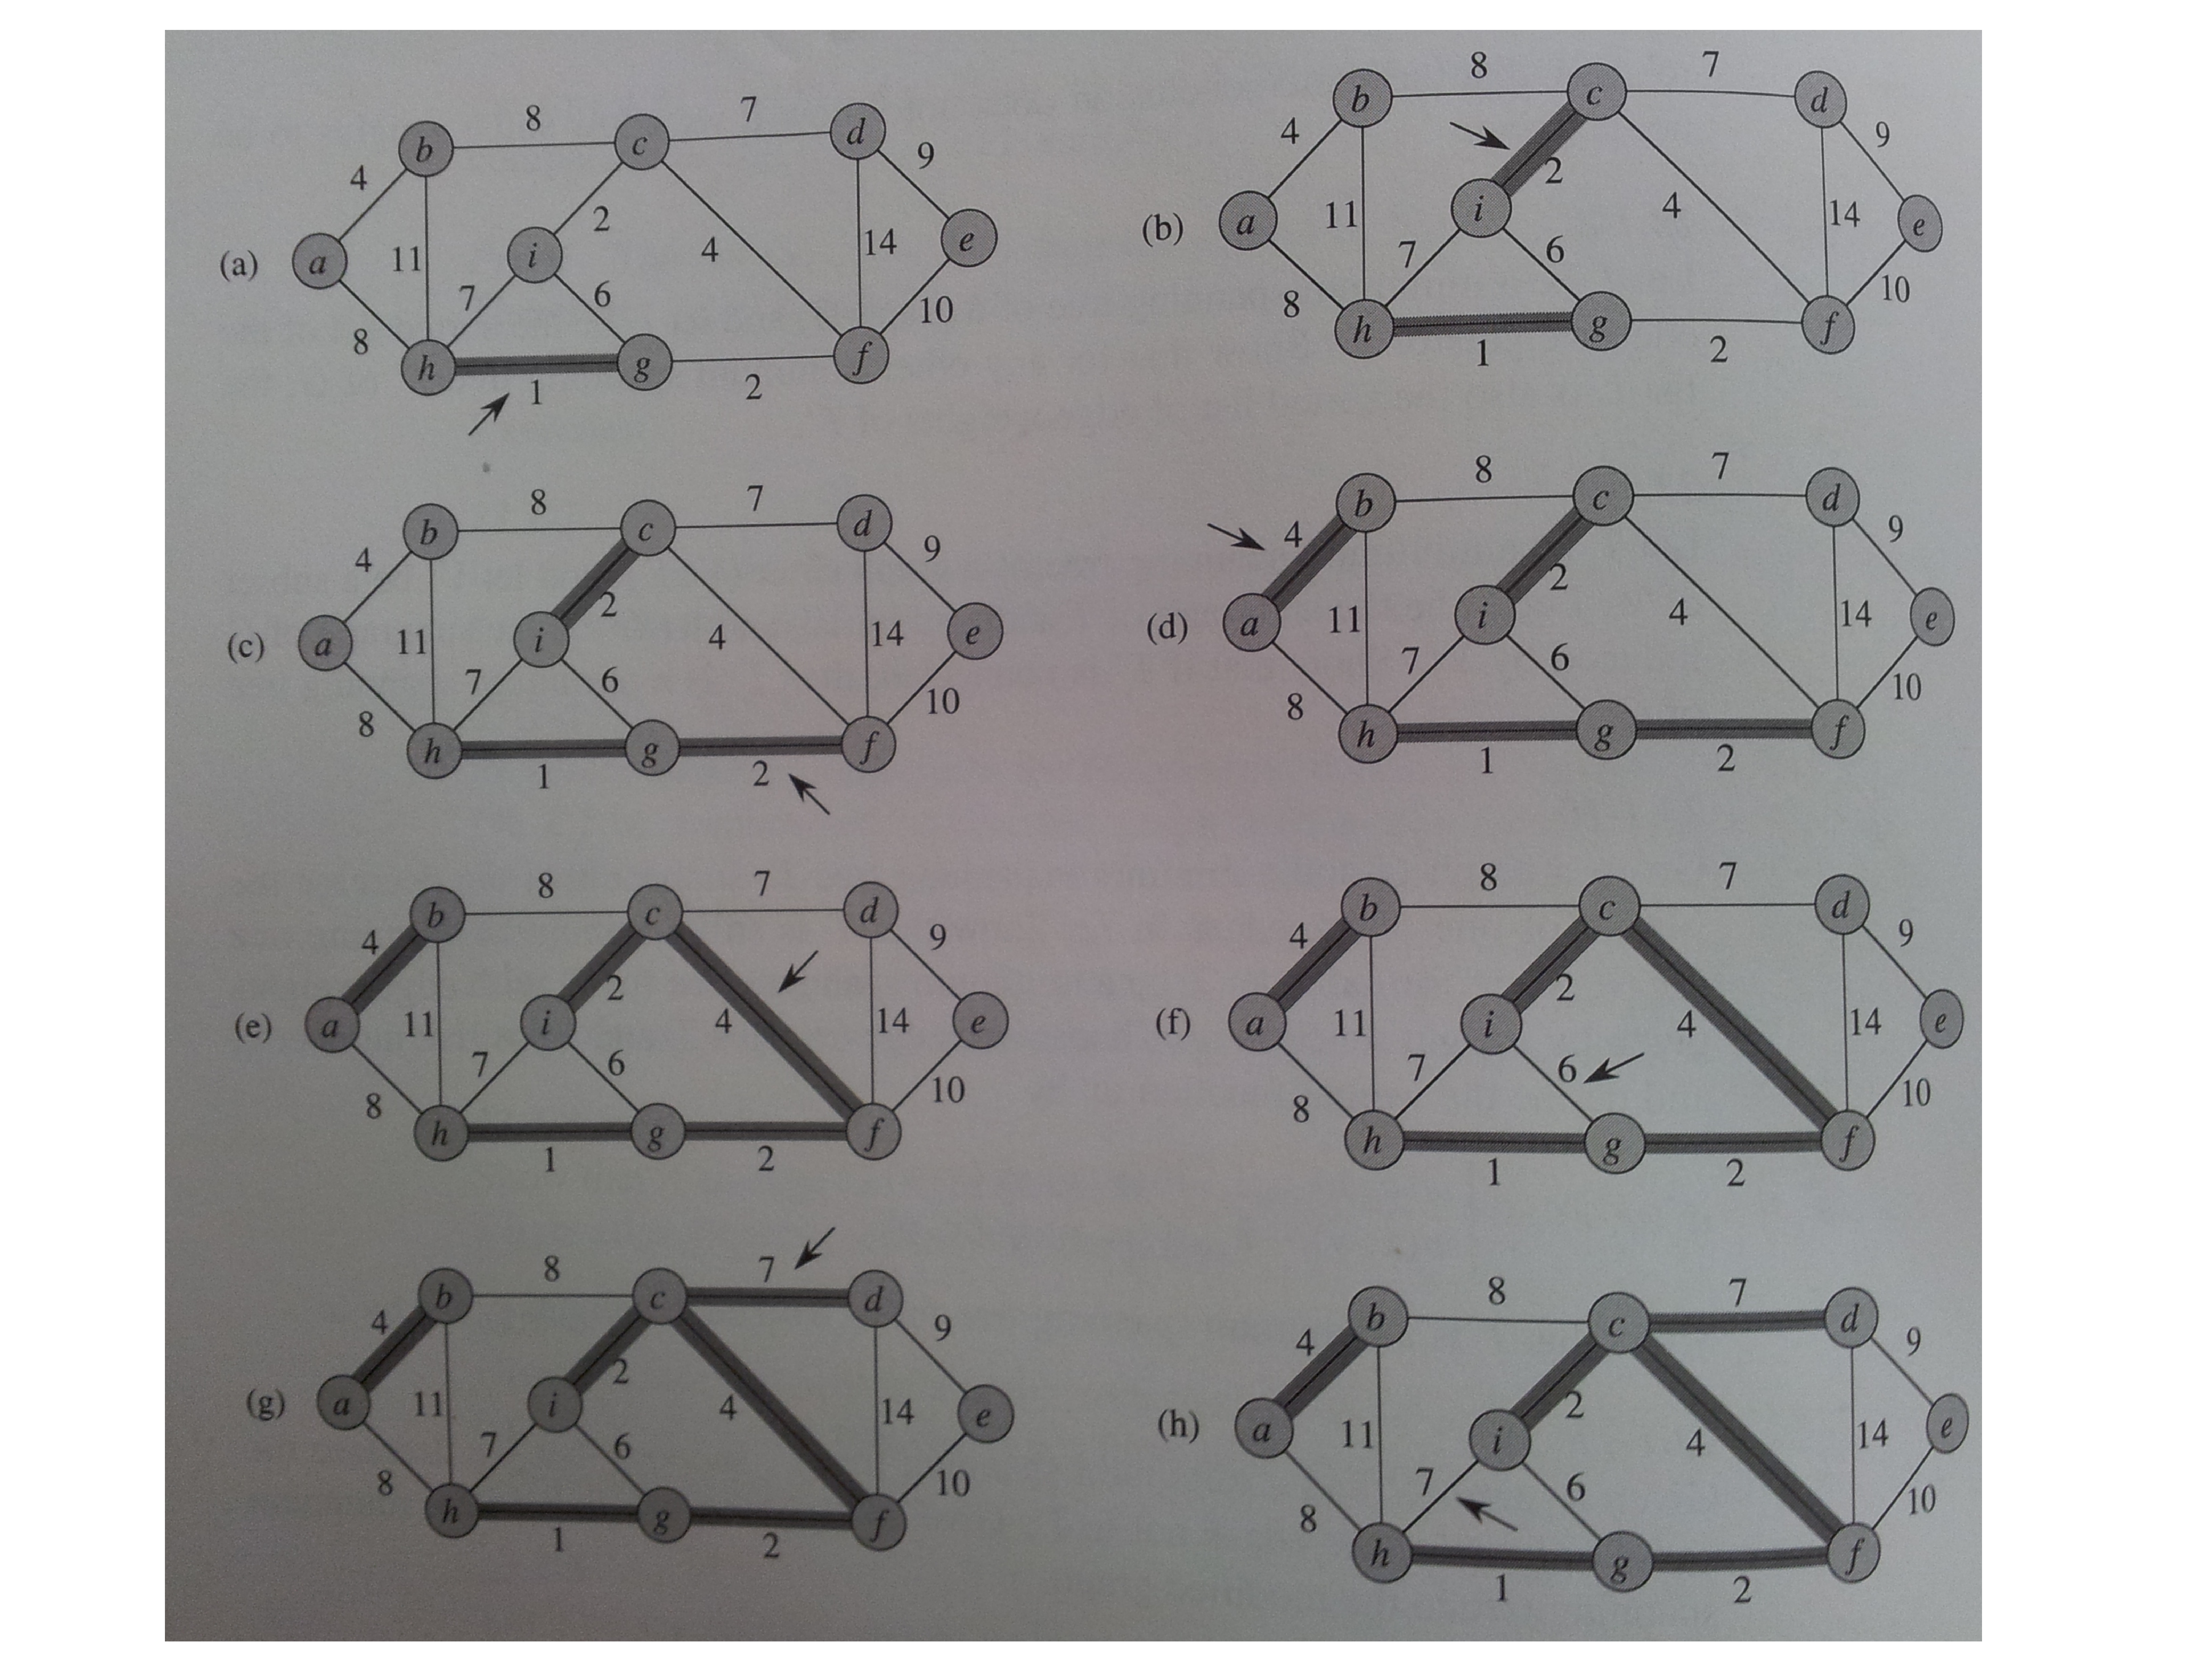
\includegraphics[width=0.7\textwidth]{greedy-figs/kruskal1.pdf}
  \end{figure}
\end{frame}

\begin{frame}
  \frametitle{Example}
  \begin{figure}[h]
    \centering
    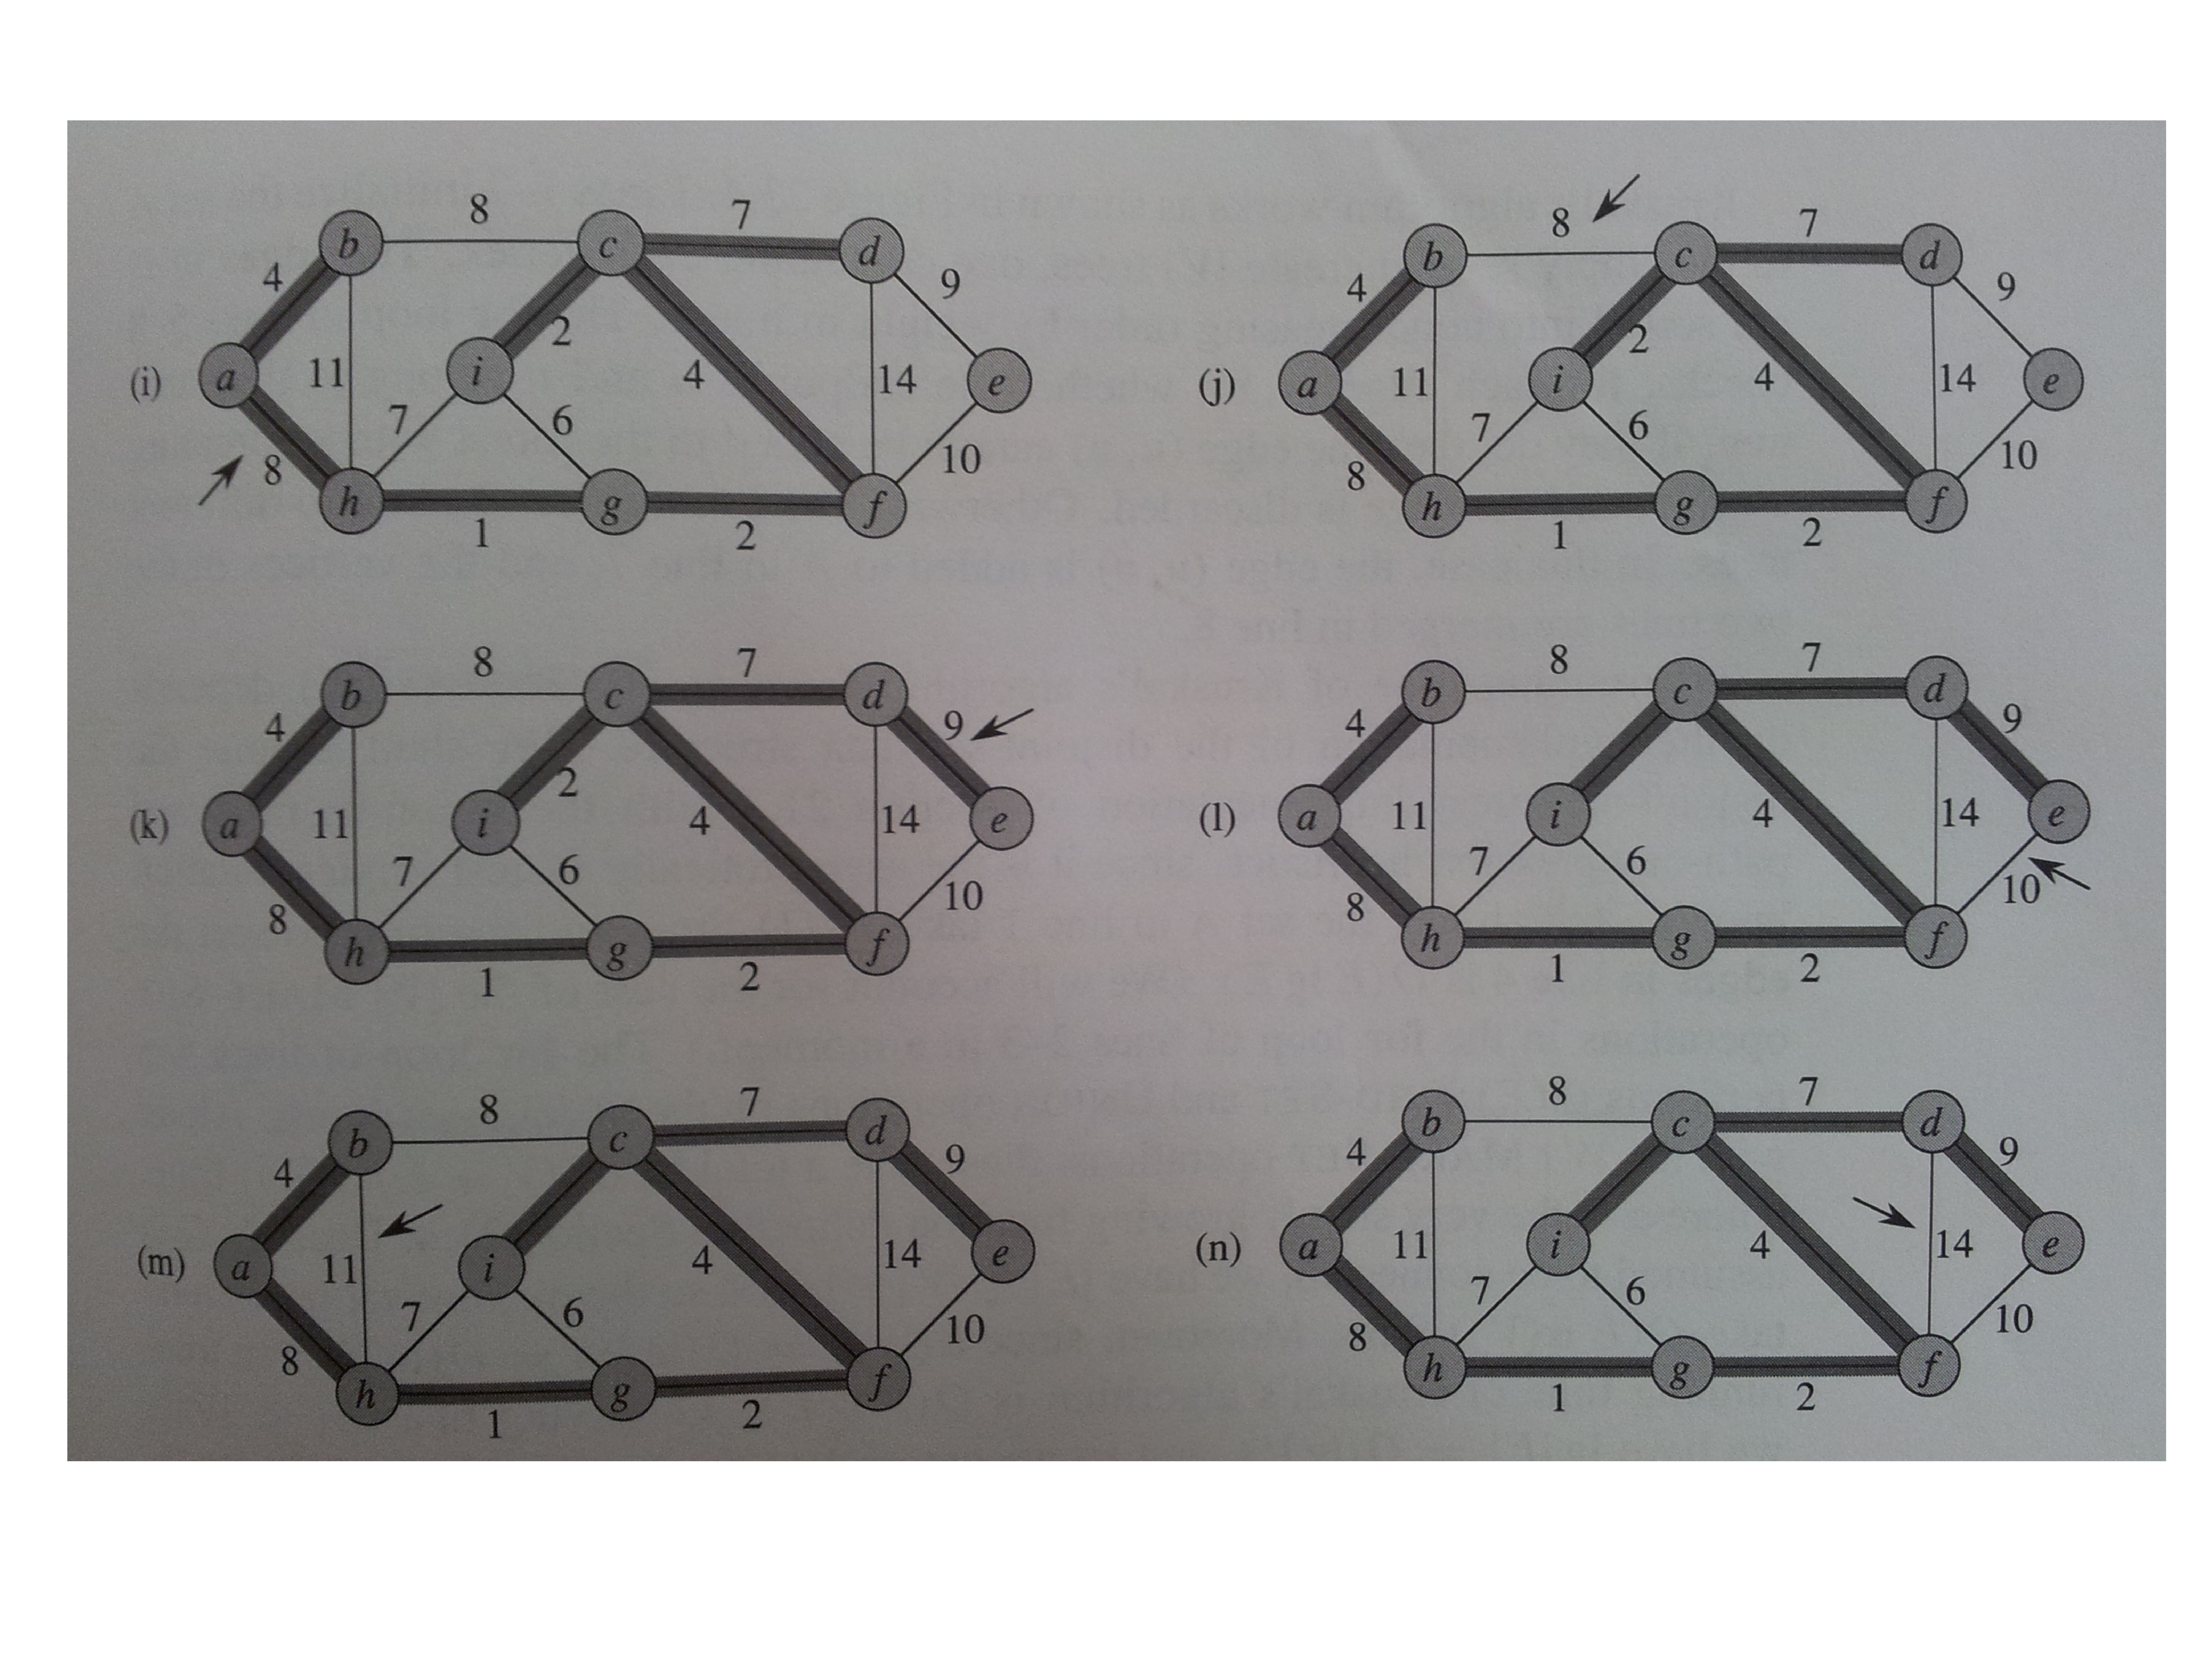
\includegraphics[width=0.8\textwidth]{greedy-figs/kruskal2.pdf}
  \end{figure}
\end{frame}

\begin{frame}

  \begin{algorithm}[H]
\SetKwFunction{KwFn}{MST-KRUSKAL(G)}
\SetKwFunction{sort}{SORT-EDGES(E)}
\SetKwFunction{findu}{FIND-SET($u$)}
\SetKwFunction{findv}{FIND-SET($v$)}
\SetKwFunction{union}{UNION$(u,v)$}

%\dontprintsemicolon
\DontPrintSemicolon
\KwFn\;
$A\gets \emptyset$\;
\ForEach{$v\in V$}{
\SetKwFunction{KwFn}{MAKE-SET(v)}
\KwFn\;
}

$F\gets$ \sort\;

\ForEach{$(u,v)\in F$}{
\If{\findu $\ne$ \findv }{
$A\gets A\cup\{(u,v)\}$\;
\union\;
}
}
\end{algorithm}
\end{frame}


% \begin{frame}
%   \frametitle{Some Definitions}
%   \begin{itemize}
%   \item Let $G=(V,E)$ be a graph with some real-valued weight function
%     $w:E\rightarrow R$.
%   \item A \textbf{cut} $(S,V-S)$ of the graph $G$ is a \textbf{partition} of $V$.
%   \item We say a cut $(S,V-S)$ \textbf{respects} $A\subseteq E$ if no edge in
%     $A$ crosses the cut.
%   \item An edge is said to be a \textbf{light edge} crossing a cut if its
%     weight is the minimum of any edge crossing the cut.
%   \end{itemize}
% \end{frame}

% \begin{frame}
%   \frametitle{This is why it works}
%   \begin{itemize}
%   \item The reason why both algorithms work is the following theorem
%     \begin{thm}
%       Let $A$ be a set of edges included in some minimum spanning
%       tree, $(S,V-S)$ a cut  that respects $A$, and
%       $(u,v)$ be a light edge crossing $(S,V-S)$. Then $(u,v)$ is safe
%       for $A$.
%     \end{thm}

%   \end{itemize}
% \end{frame}

% \begin{frame}
%   \frametitle{Correctness of Prim's Algorithm}
%   \begin{tikzpicture}
%     \path (0,0) node [draw,circle,minimum size=2.5cm]{$V-Q$};
%     \path (3,0) node [draw,circle,minimum size=2cm]{$Q$};
%     \path (2.3,0) node {$u$};
%     \draw[fill] (2.3,-0.2) circle[radius=0.05cm];

%     \path (0.7,0.5) node {$u.p$};
%     \draw[fill] (0.7,0.2) circle[radius=0.05cm];
%     \draw (0.7,0.2)-- (2.3,-0.2);

% %    \draw[fill] (0.6,-0.4) circle[radius=0.05cm];
% %    \draw (0.6,-0.4)-- (2.3,-0.2);
%   \end{tikzpicture}
%   \begin{itemize}

%  \item At the beginning of every  iteration (except the first) Prim's algorithm starts by removing    $u$ where $u.key$ is
%    minimum. This means that $(u.p,u)$ is a light edge for the cut
%    $(Q,V-Q)$
% \item Therefore Prim's algorithm is correct.
%   \end{itemize}
% \end{frame}

% \begin{frame}
%   \frametitle{Correctness of Kruskal's Algorithm}
%   \begin{itemize}
%   \item Prior to every iteration of Kruskal's algorithm we have
%     \begin{enumerate}
%     \item A forest (a collection of trees) $G_A=(V,A)$. (initially is
%       $A$ is empty)
%     \item Select an edge $(u,v)\in E-A$ with
%       \begin{enumerate}
%      \item $w(u,v)$ is minimal.
%       \item  $u\in T_u$ and $v\notin
%       T_u$ where $T_u$ is a tree in $G_A$ that contains $u$.

%       \end{enumerate}


%     \item From the above we have that: $(T_u,V-T_u)$ is a cut that
%       respects $A$ and $(u,v)$ is a light edge crossing that cut.
%     \end{enumerate}
% \item From the theorem we know that $(u,v)$ is a safe edge for $A$.
%   \end{itemize}
% \end{frame}

\begin{frame}
  \frametitle{Correctness of Kruskal's algorithm}
  \begin{itemize}
   \item Let $T=\{e_1,\ldots,e_{n-1}\}$ be the tree obtained using Kruskal's algoritm, in that order.
   \item Let $T_o$ be an mst that shares $e_1,\ldots,e_{k-1}$ with $T$ but not $e_k,\ldots,e_{n-1}$.
   \item Construct the graph $G=T_o\cup \{e_k\}$ which clearly has a cycle $C$ passing by $e_k$. 
   \item $C$ contains an edge $e\notin\{e_1,\ldots,e_k\}$ because Kruskal's algorithm does not create a cycle
   \item Furthermore $w_e\ge w_{e_k}$ because otherwise the algorithm would have chosen $e$ instead of $e_k$.
   \item Now construct the tree $T_{o_2}=T_o-\{e\}\cup\{e_k\}$ which is clearly an mst that shares $k$ edges with $T$
   \item repeating the above procedure we obtain that $T$ is an mst.
  \end{itemize}
\end{frame}
\begin{frame}
  \frametitle{Single Source Shortest Path}
  \begin{itemize}
  \item Given a graph $G=(V,E)$ with a real-valued weight function $w$
    we often as the question:
  \item What is the minimal cost (shortest)  path from $s\in V$
    to all other vertices of the graph.
  
\item First we need some definitions and theorems.
  \end{itemize}
\end{frame}

\begin{frame}
  \begin{itemize}
  \item Given a graph $G=(V,E)$ and a real-valued weight function
    $w:E\rightarrow R$.
  \item weight of path $p=(v_0,\ldots,v_k)$ sometimes written as

    \begin{align*}
      w(p)=\sum_{i=1}^kw(v_{i-1},v_i)
    \end{align*}
\item The shortest path cost $\delta$

  \begin{displaymath}
    \delta(u,v)=\begin{Bmatrix}
    \min \{w(p):u\stackrel{p}{\leadsto}v\}& \text{ if there is a path
      from u to v}\\
    \infty & \text{ otherwise }   
  \end{Bmatrix}
  \end{displaymath}
  \end{itemize}
\end{frame}


\begin{frame}
  \frametitle{Properties of Shortest Path}
  \begin{itemize}
  \item Subpaths of shortest path are subpath: Given a graph $G=(V,E)$
    and weight function $w:E\rightarrow \mathbf{R}$ let $p=(v_1,\ldots
    v_k)$ be  a shortest path from $v_1$ to $v_k$ then for any $1\le
    i,j\le k$, $p_{ij}=(v_i,\ldots,v_j)$ is a shortest path from $v_i$
    to $v_j$.
  \item \textbf{Proof}: we write $v_1\stackrel{p}{\leadsto}v_k$ which
    can be decomposed into
    $v_1\stackrel{p_i}{\leadsto}v_i\stackrel{p_{ij}}{\leadsto}v_j\stackrel{p_j}{\leadsto}v_k$
\item Then $w(p)=w(p_i)+w(p_{ij})+w(p_j)$ so if $p_{ij}$ is not the
  shortest path then $\exists p'_{ij}$ with $w(p'_{ij})<w(p_{ij})$ then
  we can write
\item $w(p')=w(p_i)+w(p'_{ij})+w(p_j)<w(p) $ a contradiction since $p$
  is the shortest path from $v_1$ to $v_k$.
  \end{itemize}
\end{frame}

\begin{frame}
  \frametitle{Negative weight}
  \begin{itemize}
  \item Even if a path contains edges with negative weight a shortest
    path can still be defined.
  \item It is undefined if the path contains a negative weight
    \textbf{cycle}.
  \item This is because we can "cross" the cycle as many times as we
    want, every time lower the cost.
 \item Therefore in the case when there is a negative cycle on a path
   from $u$ to $v$ then we set $\delta(u,v)=-\infty$ where
   $\delta(a,b)$ is the shortest path cost from $a$ to $b$.
  \end{itemize}
\end{frame}


\begin{frame}
  \frametitle{Representation of Shortest Paths}
  \begin{itemize}
  \item In all the algorithms that we will deal with, we maintain for
    every vertex $v$ its predecessor $v.p$ (which could be NULL)
  \item At \textbf{termination} $v.p$ will be the predecessor of $v$
    on a shortest path from source $s$ to $v$.
  \item We  also maintain a value $v.d$ which at termination will be
    the value of the shortest path cost from source $s$ to $v$.
  \item During the execution of the algorithm $v.d$ will be \textbf{an
      upper bound} on the value of the shortest path cost.
  \end{itemize}
\end{frame}

\begin{frame}
  \frametitle{Relaxation}
  \begin{itemize}
  \item \textbf{Relaxing} an edge $(u,v)$ means testing if we can
    improve the shortest path cost of $v$ by using the edge $(u,v)$.
  \item If we can then we update $v.d$ and $v.p$.
    \begin{figure}[h]
      \centering
      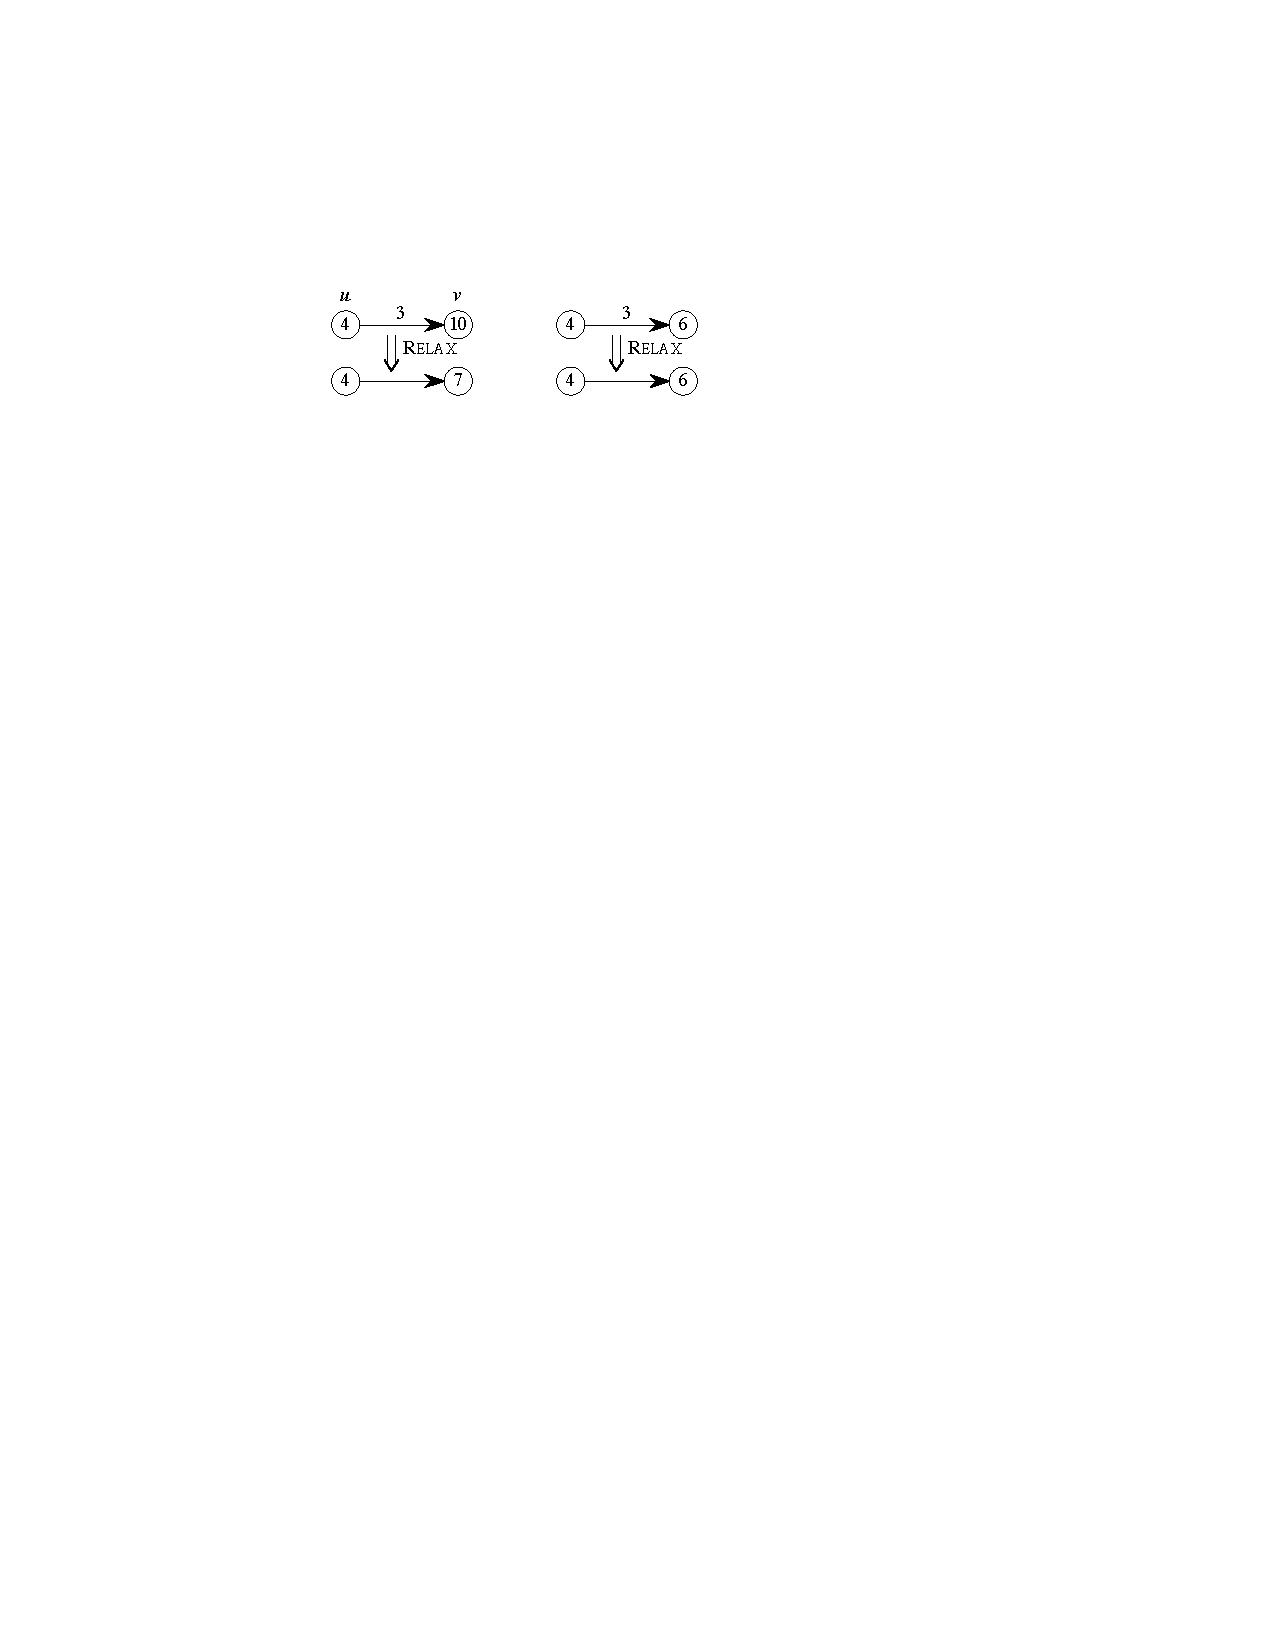
\includegraphics[width=0.7\textwidth]{greedy-figs/relax.pdf}
    \end{figure}
\item In the figure to the left the cost of $v$ was changed to the new
  cost (7) whereas to the right it was not changed since the new cost
  (7) is bigger than the current (6).
\item What is NOT shown is the change to $v.p$ in the first case.
  \end{itemize}
\end{frame}

\begin{frame}
  \frametitle{Initialization and Relaxation}
  \begin{itemize}
  \item Initially all vertices (except the source) have cost $\infty$
    and no predecessors (including the source).
  \end{itemize}
  \begin{algorithm}[H]
\SetKwFunction{init}{INITIALIZE(G,s)}
%\dontprintsemicolon
\DontPrintSemicolon
\init\;
\ForEach{$v\in V$ }{
$v.d\gets\infty$\;
$v.p\gets NULL$\;
}
$s.d\gets 0$\;
\end{algorithm}

\begin{algorithm}[H]
\SetKwFunction{RELAX}{RELAX(u,v)}
%\dontprintsemicolon
\DontPrintSemicolon
\RELAX\;
\If{$v.d> u.d+w(u,v)$ }{
$v.d\gets u.d+w(u,v)$\;
$v.p\gets u$\;
}
\end{algorithm}

\end{frame}







\begin{frame}
  \frametitle{Dijkstra's Algorithm}
  \begin{itemize}
  \item Dijkstra's algorithm is another  single source shortest path.
  \item It works when all weights are \textbf{positive}.
  \item We will see that it is faster than the Bellman-Ford algorithm.
  \item It maintains a set $S$ of nodes whose shortest paths have been
    determined
\item All other nodes are kept in a  min-priority queue to keep track of the next node to process.
  \end{itemize}
\end{frame}

\begin{frame}
  \frametitle{Dijkstra Pseudo Code}
  \begin{algorithm}[H]
\SetKwFunction{DIJ}{DIJKSTRA(G,s)}
\SetKwFunction{init}{INITIALIZE(G,s)}
\SetKwFunction{RELAX}{RELAX(u,v)}
\SetKwFunction{EXTRACT}{EXTRACT-MIN(Q)}
\DIJ\;
\DontPrintSemicolon
\init\;
$S\gets\emptyset$\;
$Q\gets V$\;
\While{$Q\ne\emptyset$ }{
  $u\gets \EXTRACT$\;
  $S\gets S\cup\{u\}$\;
  \ForEach{$v\in Adj[u]$}{
    \RELAX\;
  }
}
\end{algorithm}
\end{frame}

\begin{frame}
  \frametitle{Example}
  % \begin{figure}[h]
  %   \centering
  %   \includegraphics[width=\textwidth]{greedy-figs/example-dijkstra.pdf}
  % \end{figure}
\end{frame}

\begin{frame}
  \frametitle{Complexity}
  \begin{itemize}
  \item The running time of Dijkstra's algorithm depends on the
    implementation of the queue.
  \item Using a min-heap on a sparse graph gives complexity of
    $O((V+E)\log V)$.
  \item This is because the while loop executes $V$ times. The
    extract-min is $O(\log V)$ for a cost of $V\log V$. The relax
    includes an key update which means $\log V$. Since each edge is
    relaxed at most once then the total is $E$ with a cost of $E\log V$.
  \end{itemize}
\end{frame}

\begin{frame}
  \frametitle{Correctness}
  We show that for every iteration Dijkstra's algorithm adds node $u$ then $u.d$ is the shortest path distance from the source to $u$.
Note that the algorithm adds a node to $S$ and removes it from $Q$. Base case: initially it adds the source and $s.d=0$ which is correct.
Assume that all added nodes are such that $u.d$ is shortest path. Induction step: the next step the algorithm adds a node $v$ such that $v.d$ is minimum
among all nodes in the set $Q$ (see figure below). 
 \begin{figure}[h]
    \centering
    \includegraphics[width=0.4\textwidth]{greedy-figs/dijkstra-proof.pdf}
  \end{figure}
\end{frame}

\begin{frame}
  Suppose that the path $s\leadsto u\rightarrow v$ is not the shortest path. Then there exists a shorter
path $s\leadsto x\rightarrow y\leadsto v$. But $y.d=x.d+c(x,y)>v.d$, otherwise the algorithm would have selected $y$. Since the algorithm is used
with positive costs only then the cost of the path $s\leadsto x\rightarrow y\leadsto v$ is greater than $s\leadsto u\rightarrow v$
\end{frame}
\end{document}

%%% Local Variables: 
%%% mode: late
%%% TeX-master: t
%%%
